% Chapter 2

\chapter{Method} % Write in your own chapter title
\label{Chapter:Method}
\lhead{Chapter 2. \emph{\steel}} % Write in your own chapter title to set the page header
\begin{center}
    \textit{``Now, I return to this young fellow. And the communication I have got to make is, that he has great expectations.''}
    Charles Dickens 1861 - `Great Expectations'
\end{center}

\section{Why do we need a new modelling technique in galactic astrophysics.}
%What is missing: Massive galaxies, checks 
In this thesis we propose a new modelling technique further diversifying the range of semi-empirical models already used in the field. With the breadth of simulations and techniques already used, any additional models must justify their existence by showing they can succeed where others cannot. The primary and the arguably largest shortcoming of all the galaxy modelling techniques is the trade-off between volume and resolution. So far this limitation has severely limited the ability of models to constrain against the massive galaxy population. The reliance on discrete halos from merger trees or N-body simulations limits the number of massive galaxies simulated in more traditional models, limiting the ability of models to compare with observations of massive galaxies found in comprehensive surveys. 

%How can a new model succeed where others haven't
\steel has been designed as a \textit{complementary} tool to the other galaxy models. In this chapter we describe the gaps in the current modelling space and the design choices in \textit{steel} designed to address these gaps.

\section{Designing to specification.}
%General format: Science problem and design solution 
\subsection{Volume vs. Resolution}
%Volume/resolution - statistical
The trade-off between volume (or the number of galaxies) and resolution (the smallest element explicitly realised in the simulation) stems directly from computational limitations. High-resolution simulations resolve orders of magnitude more small haloes than large, below $10^{13.5}$ the halo number density increases by about one order of magnitude per decreasing decade in halo mass (left panel Figure \ref{fig:SubHaloes_byz}). Due to the limited computational resources available to a simulation there is an upper limit to the total number of haloes/galaxies that can be simulated. Either increasing the volume or lowering the resolution will increase the total number of galaxies simulated, and therefore one must come at the expense of the other. In Figure \ref{fig:Vol_v_Res} this is visualised showing the Baryon Mass Resolution against the Number of Galaxies for many hydrodynamical simulations. The parallel diagonal lines running from top left to bottom right are lines of constant particle number which when all other factors are constant will correspond to computational power. The two shaded boxes show the simulations that explore two modelling regimes:
\begin{itemize}
    \item The ``zoom in'', where resolution is favoured allowing for the analysis of small galaxies/haloes and the structures of larger galaxies/haloes.
    \item The ``box'', where a box of a given volume is simulated to probe the large scale structure of the Universe at the expense of resolving smaller galaxies and haloes.
\end{itemize}

\begin{figure}[h]
    \centering
    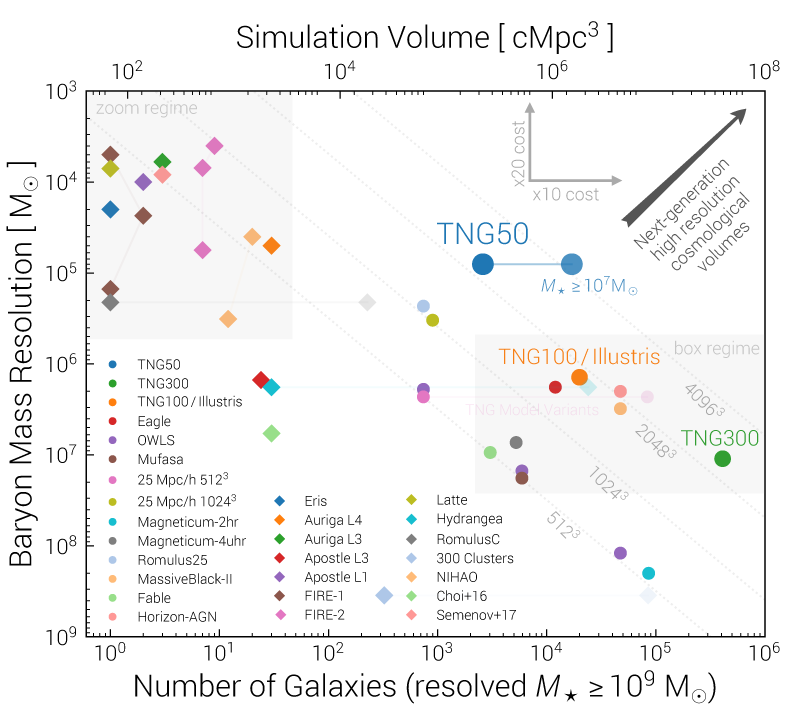
\includegraphics[width = \linewidth]{Figures/Chapter2/VolumeResolutionComparison.png}
    \caption{In this figure the positions of several simulation is volume-resolution space is shown. The vertical axis is baryon mass resolution or the size of the elements in the simulation. The horizontal axis is the simulation volume (shown on the top) which correlates with the number of galaxies (shown on the bottom). The faint grey lines running from top left to bottom right are lines of constant particle number. The two shaded boxes in the top left and bottom right show respectively the zoom and box simulation regimes. Coloured shapes are galaxy simulations as labelled. 
    Image used with permission from: Illustris-TNG Project, \citet{Nelson2019FirstFeedback}}
    \label{fig:Vol_v_Res}
\end{figure}

Semi-Analytic and Semi-Empirical models are also constrained by volume and resolution in a simmilar way. Traditionally each uses merger trees which can either be generated analytically or extracted from an N-body simulation, r
for those models that use N-body simulations directly they have simmilar constraints as in Figure \ref{fig:Vol_v_Res} but with dark matter particle resolution and number of haloes. Simply, the number of haloes on a given merger tree is directly related to the lowest mass halo of interest. However, models using merger trees have one additional level of flexibility: they can have a minimum subhalo mass and a minimum central halo mass. This provides flexibility in what can be simulated, by flexibly `pruning' the tree and removing (sub)haloes we can adapt the halo background we are using to focus computational power on important features. 

\steel has been specifically designed to overcome the limitations of volume and mass resolutions using a \textit{``Statistical Dark Matter Accretion history''} described in full in Section \ref{subsec:SDMAH}. In brief, the statistical accretion histories follow the average growth of a given mass of halo backwards in time from $z = 0$. At each time-step, t, the average number of infalling subhaloes to a given halo growth history is calculated by comparing the USHMF at t and t +$\Delta$t. The lifetime of subhaloes controlled by the input dynamical timescales. The advantage of calculating the subhalo accretion in this way is that the prerequisites are only the average halo mass growth and the USHMF, each of which have been analytically defined \cite{vandenBosch2014ComingWells, Jiang2016StatisticsFunctions}.
\steel therefore simulates massive haloes and small haloes on equal footing and is able to produce massive rare galaxies in the same run as smaller galaxies with the same precision.

\subsection{Flexibility through stability}
%Flexibility - empirical
Hydrodynamical and Semi-Analytic models are tuned for two reasons. The first is for stability, these models have tens of parameters acting in the sub-grid for hydrodynamical or as the primary modelling tool for semi-analytic models. The issue stems from multiple parameters each contributing to one galaxy variable, changing one parameter ripples throughout the model. In abstract consider a model with two parameters, $\alpha$ that controls a galaxy mass with a secondary effect on size, and $\beta$ that controls galaxy colour with a secondary effect on galaxy mass. Changing $\beta$ with the intent of modifying the colour of galaxies will force a reaction in $\alpha$ to compensate for the change in mass and then propagate into the size of galaxies. Secondly, the tuning allows fits to observations, the models are given freedom in their parameter sets to fit many galaxy properties at the same time but due to the overlap in what each physical assumption can control this leads to degeneracy in parameter space. To complicate comparison further, some models have more physical routines than others resulting in models and parameters in the less complex model compensating for this missing physics. The diversity in models and the diversity introduced by different tuning data has been extensively discussed in the literature \cite{Knebe2015NIFTyModels,Cui2018TheApplications,Knebe2018CosmicModels}.   

This degeneracy has in some part been addressed by semi-empirical models. Fundamental variables, such as galaxy stellar mass, are set using observationally-based techniques such as abundance matching (Section \ref{C2:SubSec:AbnMtch}), which remove the reliance on the physical models and parameters that are required to generate this quantity in more comprehensive/ab-initio models. `Bottom-up' modelling like this gives semi-empirical models the ability to use dramatically reduced parameter spaces and also reproduce essential observables, such as the central stellar mass function, by design. Additional physical models are added only where necessary, creating tight constraints for the core of the model and severely limiting possible degeneracies. In the semi-empirical framework, additional physical processes and associated parameters can be added in a modular fashion. For example, \citet{Shankar2014} added an analytic recipe for the size evolution of galaxies onto a network of dark matter merger trees in which central and satellite galaxies were assigned via abundance matching techniques. In the \citet{Shankar2014} SEM, the addition of the ``size evolution'' block, is completely independent of the core features of the model, namely the mass evolution of galaxies, which is fully controlled by the dark matter assembly and the input SMHM relation. This modularity of SEMs prevents degeneracies which often affect more complex, multi-parameter models. Semi-empirical models can use this to great advantage testing, for example, multiple size evolution models on one assembly background without need for re-tuning or fear of disrupting the essential results. In this thesis we extend this idea of empirical stability and flexibility further. In STEEL the backbone is of statistical nature, in which the different additional physical processes are expressed in the form of probabilistic models. These models are entirely modular and their impact on the final outputs can be individually analysed. 

It is noteworthy that some hydrodynamical cluster simulations are beginning to use a technique where haloes/galaxies are ``genetically modified''. This methods runs a simulation multiple times and making slight adjustments to the initial conditions such that the models are nearly identical aside from, for example, changing the distribution of dark matter to preference a larger merger mass ratio without changing the total simulation mass. This is a highly complementary and powerful technique that is yet to be fully realised \cite{Rey2018QuadraticHistory}.

\subsection{Consistency}
%Consistency - ensuring connections between high and low redshift
It is well documented that reproduction of the stellar mass function at multiple epochs has been a challenge for semi-analytic models \cite{Knebe2018CosmicModels, Asquith2018CosmicModels} and hydrodynamical models (although major improvements have been seen recently, for example, Illustris vs Illustris TNG \cite{Nelson2015TheRelease, Nelson2019TheRelease}). This has not however prevented such models from making bold claims about the successes of their models in terms of morphology and mass assembly without providing a full stellar mass function history \cite[e.g.][]{Somerville2008ANuclei, Hopkins2010MERGERSMATTER}\footnote{A merger history matched to an observational merger history as provided by \citet{Hopkins2010MERGERSMATTER} is insufficient as we show in Chapter \ref{Chapter:GalPairs} the methods involving pair fractions used to estimate these rates have a large degree of systematic error.}. As an example, a kettle at temperature A is modelled to cool under an arbitrary physical model $\gamma$, to temperature B in time T. If A is observed to be false compared to the data, and B is observed to be consistent with the data, than the inference that $\gamma$ is a correct physical model is baseless. Galaxy models that fail to reproduce the stellar mass function at high redshift repeatedly invoke this kind of logic when the $z=0$ stellar mass function is reproduced. An overabundant stellar mass function at high redshift that evolves to the observed stellar mass function at low redshift, implies either lack of growth in the galaxy population to allow the observed stellar mass function to catch up, or over-merging of galaxies to reduce the total number density. A semi-empirical model designed to faithfully reproduce the time-dependent stellar mass function and the distribution of satellite galaxies, as the foremost modelling priority has a major advantage. 

\subsection{Speed}
%Systematics - speed

Speed is a critical ingredient in any model. Hydrodynamic models have run-times of months using millions of CPU hours, and semi-analytic models constrain highly-multi dimensional parameter space for thousands of merger histories. In each case high speed is critical to the models reaching conclusions in reasonable time frames. Semi-empirical models are faster by design. Characterised by smaller parameter spaces, they can leverage more computational time to explore physical models or take advantage of larger simulation boxes. 

By using a \textit{``Statistical Dark Matter Accretion history''} and forgoing discrete haloes/merger trees \steel's run time is dependent on different factors to other models; the width of the mass bins used for the halo and subhalo mass functions (which corresponds to the resolution of haloes), and the computational complexity of any physical modelling routines. As \steel is not tuning parameters in high dimensional space or applying physical models one by one to thousands of discrete merger trees, it can instead leverage computational power to test combinations of internal physical models or be run on more modest, cheaper, and widely accessible hardware.

\section{Modules and Methods}

\subsection{Statistical Dark Matter Accretion History}
\label{subsec:SDMAH}

Fundamentally, the single most important element of \steel and a large part of what makes it unique, enabling an alternative view of galaxy formation problems, is the \textbf{\textit{statistical dark matter accretion history}}. As described above, a large part of the power of \steel come from the removal of discrete merger trees or haloes. We provide here a discussion of N-body and processed merger trees building upon Section \ref{sec:LCDM} followed by a detailed description of how the statistical dark matter accretion history is constructed.

%First we should explain merger trees and traditional simulation techniques.
\subsubsection{Traditional methods and merger trees}

%first n body

The state of the art in dark matter modelling is N-body simulations. N-body models simulate billions of individual particles, computing the acceleration and updating the position for each particle over thousands of time-steps. They calculate the evolution of dark matter from the distributions that mirror that of the cosmic microwave background, to the cosmic web of haloes and filaments inferred from observations of galaxies today. The non-interacting nature of \textbf{cold} dark matter allows for only gravitational force to be considered; thus modern dark matter simulations are able to leverage the massive power gains made recently in GPU computing allowing for ever larger and higher resolution dark matter only simulations to be run. 

The outputs of even the previous generation n-body dark matter simulations, such as the Bolshoi simulation a snapshot of which is shown in Figure \ref{fig:Bolshoi}, total tens of gigabytes for individual $50 Mpc^3$ sections and terabytes to capture the whole $250 Mpc^3$ simulation. To use all of this information would be impractical for any galactic modeller without access to high-performance computing hardware and a good understanding of memory management. Furthermore, despite the excellence provided by halo-finders and merger tree extractors such as \textsc{rockstar} \cite{Behroozi2011TheCores} and the `consistent trees' algorithm \cite{Behroozi2013GRAVITATIONALLYCOSMOLOGY}, the merger trees are frequently not fit for use in models unless specifically built to handle these inputs. Finally, as discussed by van den Bosch \cite{vandenBosch2014ComingWells, vandenBosch2017DissectingSimulation, vandenBosch2018DisruptionFiction}, the interpretation of dark matter simulations is of vital importance; both the analysis tools and the fundamental design decisions taken when building the simulation, have systematic effects on the outputs all which complicate comparison between simulation outputs e.g. subhalo statistics, velocity fields, etc.

\begin{figure}[h]
    \centering
    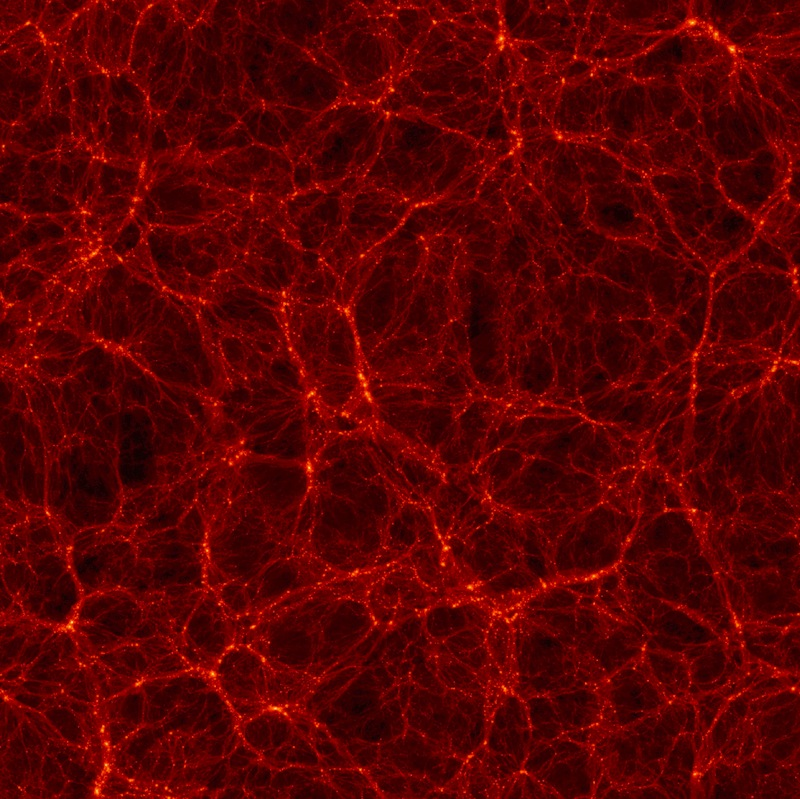
\includegraphics[width = \linewidth]{Figures/Chapter2/Bolshoi.jpg}
    \caption{Snapshot of the 250 Mpc$^3$ box of the Bolshoi Simulation. Brighter regions indicate a higher density of dark matter. Note the clustered bright points connected by large filaments. This structure is known as the cosmic web.
    Image credit: Bolshoi Simulation http://hipacc.ucsc.edu/Bolshoi/Images.html}
    \label{fig:Bolshoi}
\end{figure}

The choice of many analytic and empirical models to instead opt for analytically derived Press Schecter trees that can be generated `on-the-fly' or pre-processed comes from the simplicity and flexibility afforded by this technique. However, trees generated in this way are still affected by volume (i.e. number simulated) and resolution (i.e. size of the smallest halo accounted for in any split) limiting there effectiveness.

\subsubsection{State-of-the-art statistical method}
%then get onto what makes STEEL STEEL
\begin{figure}[h!]
    \centering
    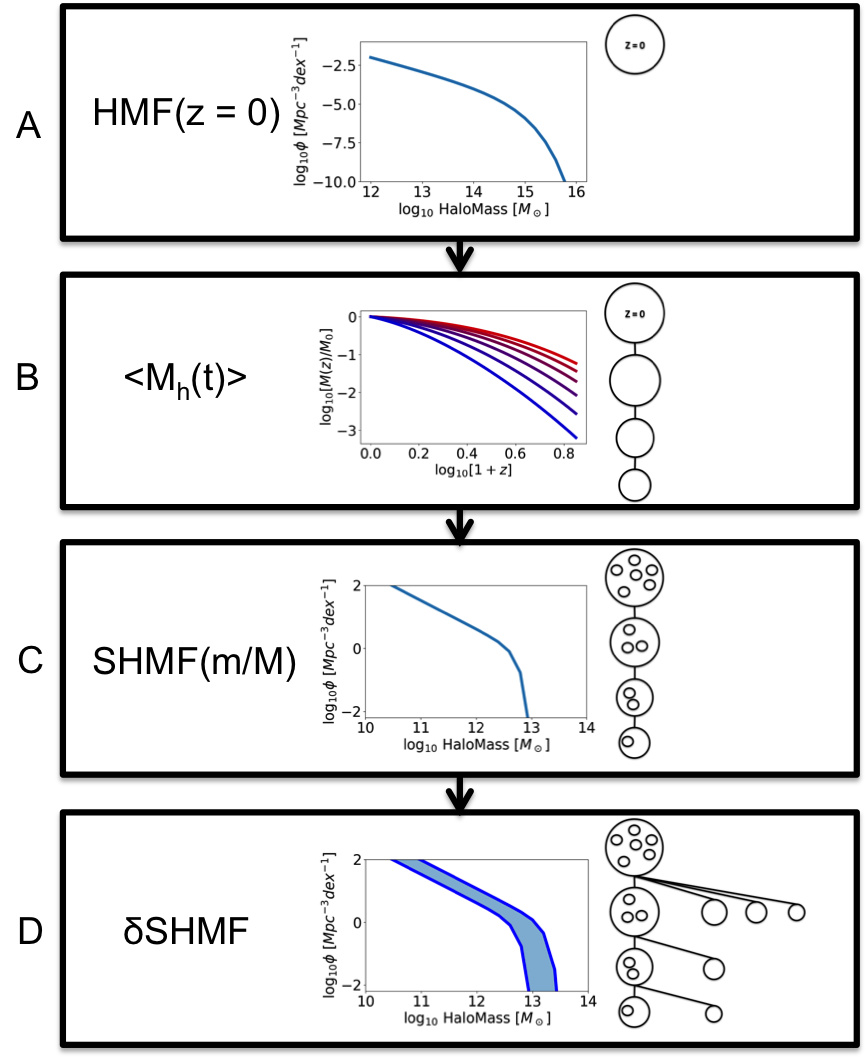
\includegraphics[width = \linewidth]{Figures/Chapter2/StatDM.png}
    \caption{We show the main steps in building the statistical dark matter accretion history for STEEL. Each panel shows a feature from a traditional merger tree and the statistical function used to replace it. A: The HMF is used to calculate the number densities of central haloes. B: Average mass growth histories are used to calculate the size of each mass bin at previous epochs. C: The (unevolved) SHMF is used to populate each central at each redshift with subhaloes. D: The average number densities of accreted subhaloes at each epoch are calculated by taking the difference between each mass bin of the (unevolved) SHMF at consecutive redshift steps.}
    \label{fig:StatDM}
\end{figure}

The core principle of the statistical methodology is to treat parent haloes and satellites galaxies/haloes as ``average'' populations, avoiding the issues with volume and resolution as described previously. Here we detail the step-by-step construction of the statistical dark matter accretion history complemented with a graphic representation in Figure \ref{fig:StatDM}.

\textbf{Central Haloes}

We start by considering a fine grid of central dark matter haloes ranging from $M_{h}=10^{11}\, M_{\odot}$ to $M_{h}=10^{15}\, M_{\odot}$ at redshift $z=0$. Their number densities are given by the halo mass function (HMF) of \citet{Despali2016TheDefinitions}, which is obtained using the COLOSSUS Python package \citep{Diemer2018COLOSSUS:Halos}. COLOSSUS also contains spherical over-density conversions required throughout this work, as well as many other halo mass functions which may be switched to or from to test different cosmologies as the statistical dark matter accretion history is theoretically independent of may of the choices.

The halo mass function provides the number densities of haloes in a given mass bin (Figure \ref{fig:StatDM}, Panel A).
The average mass growth histories of all main progenitors in the bin of halo mass $[M_{h},M_{h}+dM_{h}]$ are then calculated using the analytic model from \citet{vandenBosch2014ComingWells}\footnote{This model further improves on the seminal work by \citet{Parkinson2008GeneratingTrees}, which was aimed at reproducing numerical merger trees, optimised with small redshift steps minimising the development of systematic errors at late cosmic epochs.}. This provides the average ``main progenitor'' branch of a traditional merger tree for each mass bin at $z = 0$ (Figure \ref{fig:StatDM}, Panel B.)

\textbf{Assigning Subhaloes to Parent Haloes}

In order to predict the number of satellite galaxies, we must associate to each parent/central halo the number and mass of subhaloes they are expected to contain. To achieve this we use the subhalo mass function (SHMF). The SHMF describes the expected distribution of subhaloes of mass $M_{h,sat}$ in a given parent halo of mass $M_{h,cent}$, as a function of $M_{h,sat}/M_{h,cent}$. Multiple definitions for the SHMF exist depending on the way a subhalo is defined. In this work we use two definitions of the SHMF. The first is the unevolved SHMF (USHMF), which describes the total subhaloes accreted over a parent halo's lifetime. In the unevolved SHMF any merging or stripping in the subhaloes occurring after infall is ignored. Several groups have been able to constrain the unevolved SHMF \citep{Giocoli2008AnalyticalHaloes,Jiang2016StatisticsFunctions}. In what follows, we use a recent rendition of the unevolved SHMF by \citet{Jiang2016StatisticsFunctions}, which is calibrated against the Bolshoi simulation\footnote{We direct the interested reader to \citet{Jiang2016StatisticsFunctions} for further discussion of the unevolved SHMF as well as of other SHMFs, such as the evolved SHMF where the number densities are affected by both subhalo stripping and mergers.}.

The second definition we use in this work is the unevolved ``surviving'' SHMF (USSHMF). Subhalo masses are assumed ``frozen'' at infall but the subhalo number densities can reduce compared to the unevolved SHMF as the unevolved surviving SHMF accounts for subhalo disappearance due to merging with the parent halo. Subhalo merging is due to loss of angular momentum to the parent halo via `Dynamical Friction' described in Section \ref{subsub:DynF}. We show in Figure \ref{fig:SHMF_clus} for a representative parent halo of mass $\log M_{h,cent} M_{\odot} = 12.80$, the unevolved SHMF and three unevolved surviving SHMF characterised by different dynamical friction timescales $\tau_{dyn}$. Larger $\tau_{dyn}$ lead to a milder reduction in subhalo number densities as subhaloes take longer to merge with the parent halo. Lower $\tau_{dyn}$ are less effective in reducing the number densities of smaller subhaloes which are more likely to have dynamical friction timescales comparable to or larger than the Hubble time at $z = 0$.
\begin{figure}[h!]
    \centering
    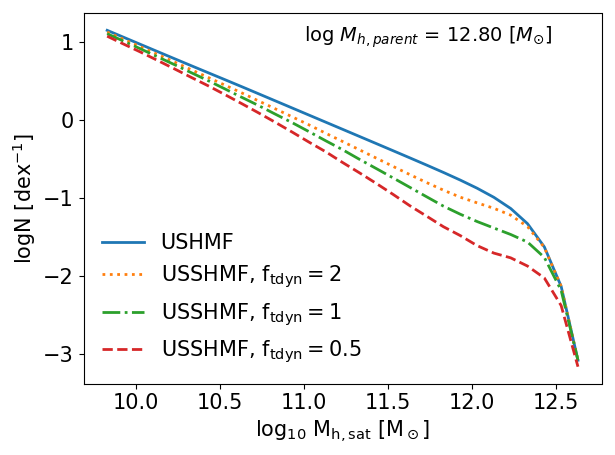
\includegraphics[width = \linewidth]{Figures/Chapter2/SHMF_OneCluster.png}
    \caption{Comparison between the unevolved SHMF (solid line) and three unevolved surviving SHMF  (dotted lines) for a parent halo of mass $\log$ $M_{h,parent}$ $[M_{\odot}] = 12.80$. The factor $f_{t_{dyn}}$ is applied to the merging timescales of the haloes. Lower factors correspond to lower unevolved surviving SHMF where more subhaloes have merged.}
    \label{fig:SHMF_clus}
\end{figure}

\textbf{Average Subhalo Accretion}

At each redshift step along with the mass growth histories, we calculate the unevolved SHMF associated to the parent halo mass. This is equivalent to the substructure found in traditional merger trees (Figure \ref{fig:StatDM}, Panel C). However, unlike traditional methods, our statistical approach is able to probe ``rare'' subhaloes without running prohibitively large volumes of merger trees.

For each time step we can now calculate a mass function describing the number density of subhaloes accreted onto the population of central haloes in the halo mass bin $[M_{h,cent}(z),$ $M_{h,cent}(z) + dM_{h,cent}(z)]$, which is computed by differentiating the unevolved SHMF across two neighbouring redshift steps $z$ and $z+dz$. In practice we can calculate the average number density of subhaloes of any given mass $M_{h, sat}$ that are accreted in the redshift interval $dz$ onto the main progenitor haloes with mass in the bin $[M_{h,cent}(z),$ $M_{h,cent}(z) + dM_{h,cent}(z)]$ as,
\begin{equation}
\label{eqn:deltSHMF}
\begin{split}
&\delta USHMF[z, M_{h,cent},M_{h,sat}] =  \\
&USHMF\Big(\frac{M_{h,sat}}{M_{h,cent}(z)}\Big) - USHMF\Big(\frac{M_{h,sat}}{M_{h,cent}(z + \delta z)}\Big).
\end{split}
\end{equation}
In this way the unevolved subhalo accretion history ($\delta USHMF$) is retrieved for all main progenitor haloes at all redshifts.

\subsubsection{Dynamical Friction}
\label{subsub:DynF}
Dynamical Friction is the process by which an object (particle) moving though a mass `field' (or distribution of particles) loses velocity and increases the velocity of the field via gravitational interactions. A simplified example is shown in Figure \ref{fig:Tdyn_toon}; the red particle is initially moving to the left between two rows of particles of infinite extent that interact only though gravity (and only with the red particle). The particle in Panel A receives an equal pull from all particles and therefore experiences no acceleration. The black particles directly above and below the red are the most strongly attracted and therefore move the greatest distance toward the red, with particles further away moving less proportionally to their distance. By Panel B the red particle has moved to the left and due to the previous effects now has more mass clustered it along the path. The break in the symmetry exerts a net force on the red particle in the opposite direction to its motion. In Panel C where more black particles have been drawn behind the red the effect is magnified and the resultant force strongly opposes the motion. 

\begin{figure}[h!]
    \centering
    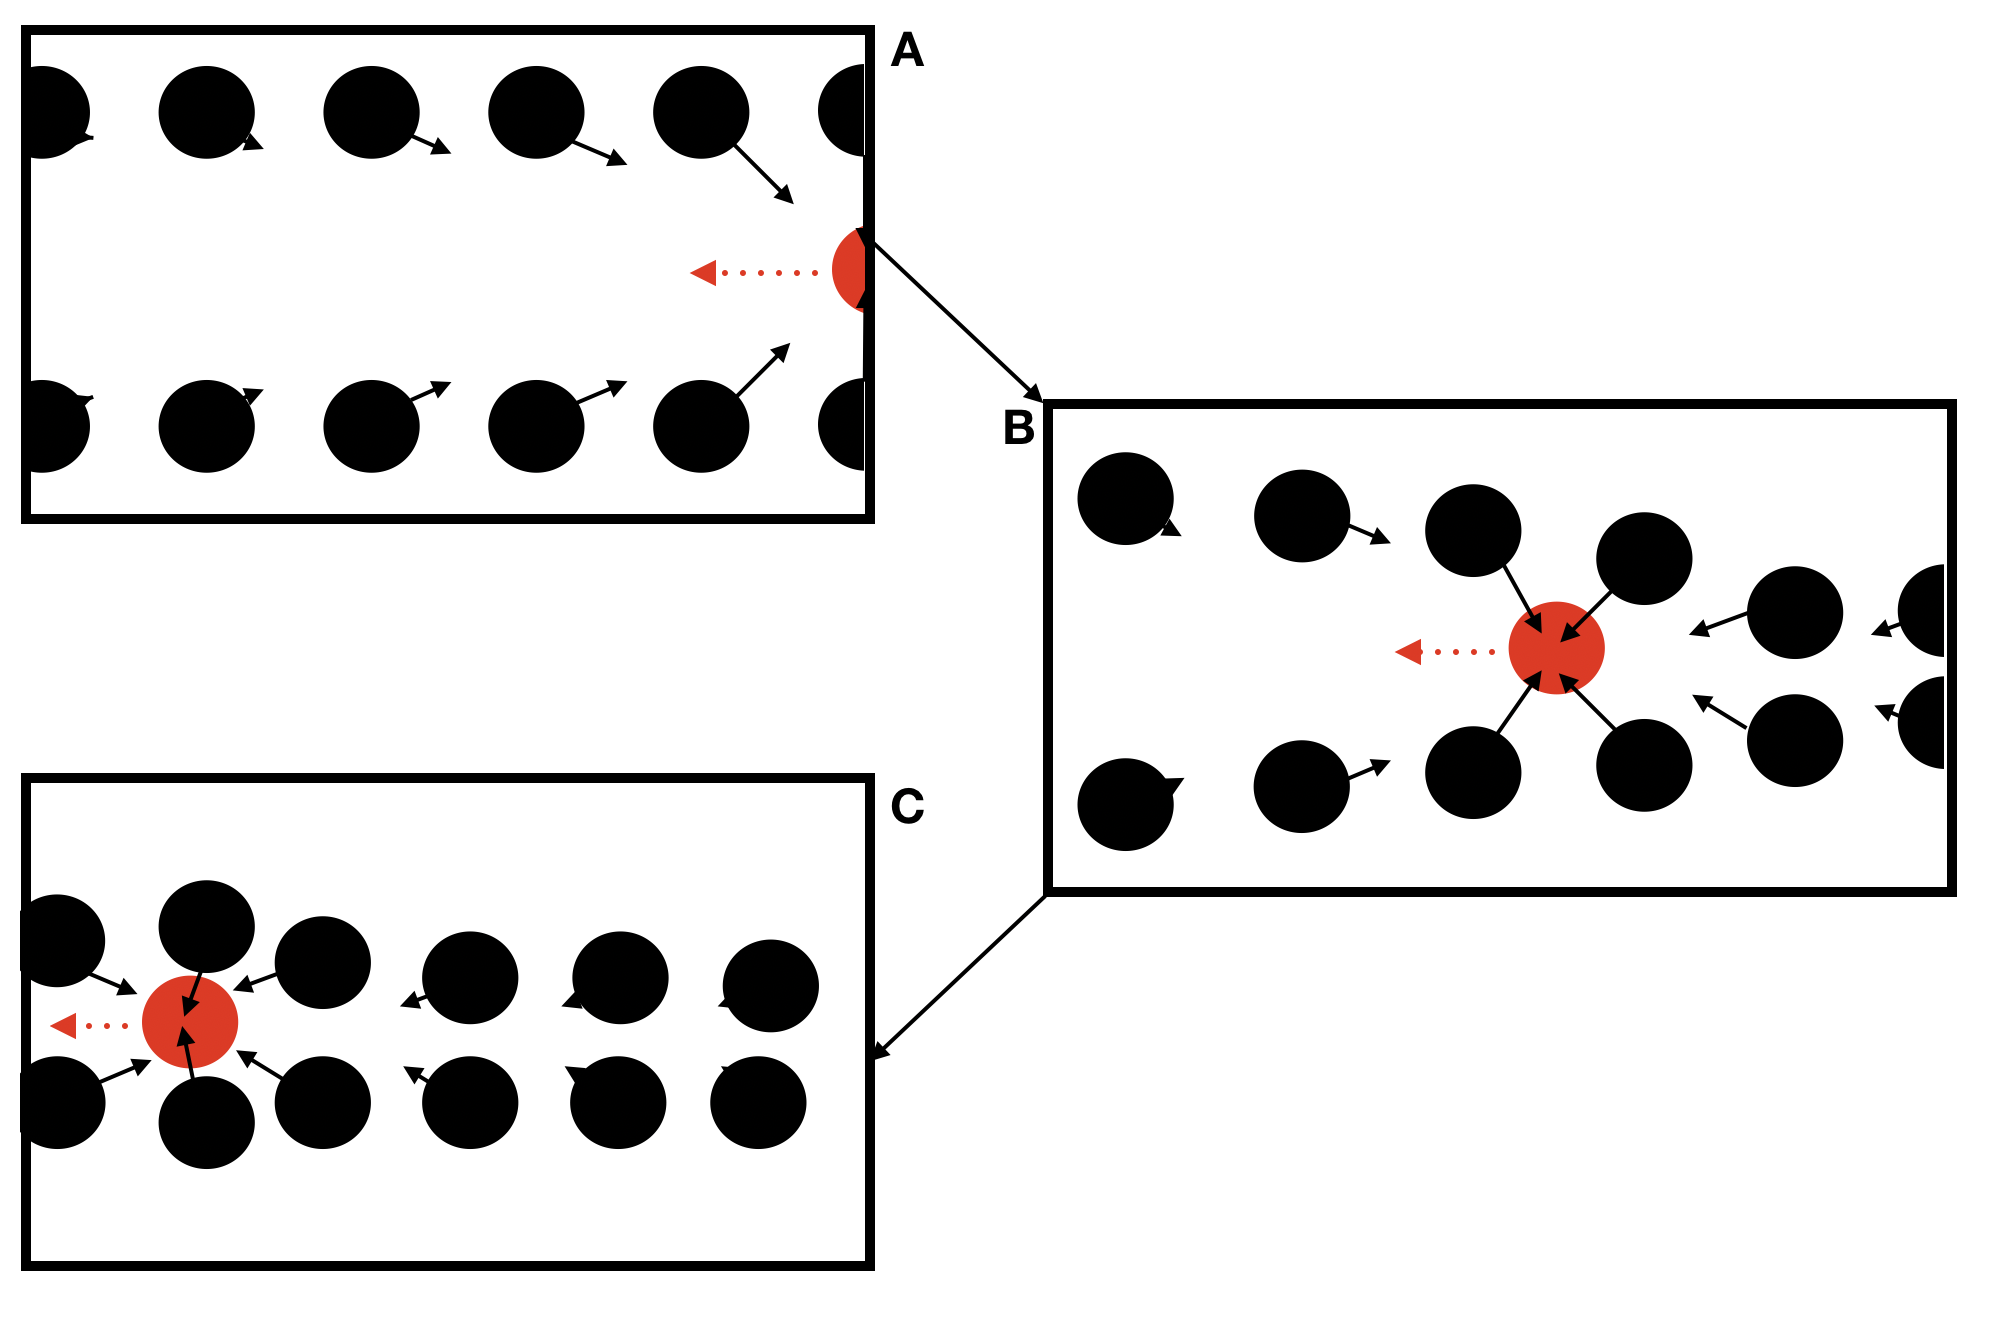
\includegraphics[width = \linewidth]{Figures/Chapter2/Dynamical_Friction.png}
    \caption{In this handmade cartoon, we depict a thought experiment to demonstrate the process of dynamical friction. We show a red test particle moving through two rows of black particles that are infinite in extent. The particles interact only though an attractive force that reduces with distance akin to gravity. The black particles interact only with the red particle and not with each other. The black particles start at rest and the red particle starts with some arbitrary velocity to the left. The panel A shows the starting configuration of the particles, the panels B and C show two theorised later states of the system. For an animation of a simulation designed around this thought experiment see: \url{https://twitter.com/RSEGrylls/status/1229104848643198979} (made and shared by PJG)}
    \label{fig:Tdyn_toon}
\end{figure}

As a descriptive thought experiment this case achieves several of the properties dynamical friction has well:
\begin{itemize}
    \item The red particle experiences a `drag' force due to the particles it draws in behind it, eventually loosing most of its momentum.
    \item The particles are non-interacting aside from gravity, as are the leading dark matter theories.
    \item The energy of the red particle is dissipated into the velocities of the black particles, the motion of a galaxy though a dark matter field increase the random motion of the dark matter.
\end{itemize}
The main features missing from the thought experiment are:
\begin{itemize}
    \item The dark matter field is not uniform and in-fact are a virialised potential well with more mass in the centre and the distributions and velocities of particles within this field are random within this distribution.
    \item The red `test' particle is in-fact a distribution of masses that are gradually lost to the field.
    \item The red particle moves in an orbit around the centre of the potential well and is stripped of mass, velocity, and momentum.
    \item The dark matter is self interacting under gravity and there is baryonic matter that interacts via processes other than gravity, although these tend to be of a lower order.
\end{itemize}



\section{Utilised Data}

In this thesis we use the stellar mass functions defined below, along with the halo mass functions, to constrain the SMHM relationship. In addition to the SMF to constrain the model at high redshifts we use measurements of massive clusters to constrain the satellite galaxy distributions.

\subsection{Stellar Mass Functions}
\label{subsec:SMF}

\subsubsection{Low Redshift, $z = 0.1$}
\label{subsub:SDSS}
At low redshift we use the Sloan Digital Sky Survey Data Release 7 (SDSS-DR7) from \citet{Meert2015ASystematics}.
The data from the SDSS-DR7 spectroscopic sample \citep{Abazajian2009THESURVEY} contain $\sim 670,000$ galaxies fitted with a S\'ersic + exponential model \citep[PyMorph;][]{Meert2015ASystematics} with associated halo masses and central satellite classifications from \citep{Yang2012EvolutionHalos}. The improved photometric analysis by \citet{Meert2015ASystematics} provides more reliable estimates of the stellar mass function at the high mass end which are more abundant than previous estimates \citep{Bernardi2016TheEvolution, Bernardi2017ComparingLight}.
In this thesis the effect of the enhanced high mass end on galaxy assembly is investigated. We compare to previous determinations of the stellar mass function using as an example the de Vaucoulers \citep{deVaucouleurs1948RecherchesExtragalactiques} based cmodel fits from SDSS \citep{Abazajian2009THESURVEY}. The latter definition of galaxy stellar mass has been extensively discussed not to be accurate, partially due to incorrect sky subtraction and adoption of non-ideal light profiles \citep{Bernardi2013TheProfile}. \citet{Bernardi2017ComparingLight} have clearly shown that the choice of light profile is not a simple matter of ``semantics''. The single or double S\`ersic models perform better in fitting the surface brightness of galaxies independently of the galactic environment \citep{Meert2015ASystematics}. The performance is thus not related to the inclusion of the intra-group or intra-cluster light in the fit \citep{Bernardi2017ComparingLight}.

\subsubsection{High Redshift, $z > 0.1$}
\label{subsub:Davidzon}
At higher redshift (0.3 \textless z \textless 3.3) we use stellar mass functions from the COSMOS2015 catalogue \citep{Davidzon2017TheSnapshots}. Here masses are defined using spectral energy distribution fitting, including ultra-deep infrared photometry. \citet{Davidzon2017TheSnapshots} use \citet{Bruzual2003Stellar2003} stellar population synthesis models to estimate stellar masses. As SED fitting is notably different from light profile fitting, one cannot apply the same corrections as in \citet{Mendel2014ASURVEY}. 
Nevertheless, to match the mass-to-light ratios adopted by \citet{Mendel2014ASURVEY}, based on the \citet{Bell2003TheFunctions} mass-to-light ratios, we follow \citet{Bernardi2013TheProfile} and increase the \citet{Davidzon2017TheSnapshots} stellar masses, based on \citet{Bruzual2003Stellar2003}, by +0.15 dex. We note that the resulting $z=0.37$ stellar mass function after this correction is in remarkable good agreement with the $z=0.1$ stellar mass function by \citep{Bernardi2013TheProfile}. Our result also matches the findings by \citet{Bernardi2016TheEvolution}, who showed that, by making use of the BOSS sample, the stellar mass function shows negligible number density evolution up to $z \sim 0.5$.

\label{subsec:Clusters}
\subsubsection{Cluster at z = 2.5, Wang+ 2016}
\label{subsubsec:Wang}
The highest redshift cluster we compare to is a $M_{vir} = 10^{13.7} M_{\odot}$ halo containing 15 galaxies with $M_* > 10^{10} M_{\odot}$ at a redshift of $z = 2.5$.
This cluster is reported in \citet{Wang2016DISCOVERY2.506}, and we provide a brief description of the observation and data here.
The cluster is observed using IRAM-NOEMA, VLT-KMOS, VLA, XMM-Newton and Chandra for the spectroscopic observation and redshift determination.  
The galaxy masses are determined assuming a \citet{Salpeter1955TheEvolution.} IMF, which we correct to a \citet{Chabrier2003GalacticFunction} IMF, by decreasing the stellar masses by 0.24 dex.
The halo mass ($M_{vir} \sim 10^{13.93} M_{\odot}$) of the cluster is estimated in three different ways, using the total X-ray luminosity, the velocity dispersion of its member galaxies above $M_* = 10^{10.76} M_{\odot}$, and the stellar richness of the cluster \footnote{We note the velocity dispersions and X-ray luminosity estimations give the cluster mass as $M_{vir} = 10^{13.73} M_{\odot}$ and the estimate given by mass richness is significantly higher $M_{vir} = 10^{14.6} M_{\odot}$, whilst we used the published average the lower cluster mass excluding the richness estimate is in as-good or better agreement with model results.}. Given this object was a targeted cluster, we cannot estimate the cosmic abundance (i.e, the number per cubic megaparsec). For analysis and comparison later in this work we assign this cluster an abundance of $N(> M_*=10^{13.93})=10^{-7.15}$ $[Mpc^{-3}]$ which is estimated by integrating the halo mass function in the limits [$10^{13.93}$, $\infty$], thus providing an upper limit to the number densities associated to clusters of this mass. 

\subsubsection{1959 Clusters at z = 0.7 - 1.0, Wen \& Han 2018}
\label{subsubsec:1959}
We compare to the cluster sample from \citet{Wen2018ARedshifts}, which contains 1959 clusters from SDSS-DR14 \citep{Abolfathi2017TheExperiment} and the WISE survey \citep{Wright2010THEPERFORMANCE}. The clusters are identified in the W1 band, and foreground objects are removed using the SDSS photometric data. The cluster mass and richness are estimated using the total W1 band luminosity within 1 Mpc of the central galaxy. As performed above, to each cluster we assign an upper limit to their abundances from the cumulative integration of the halo mass function.

\subsection{Abundance matching}
\label{C2:SubSec:AbnMtch}
In this work we populate dark matter haloes with galaxies using the abundance matching technique where galaxies are assigned to haloes by comparing the relative abundances of galaxies and haloes. For example in Figure \ref{fig:Abn_Toon} the horizontal lines connect points of constant number density between the HMF (red, top left) and the SMF (green, bottom right). Halo/stellar masses with corresponding number density are then used to define a mapping between the masses, this connection is called the stellar-mass-halo-mass (SMHM) relationship (black, bottom left).

\begin{figure}[h]
    \centering
    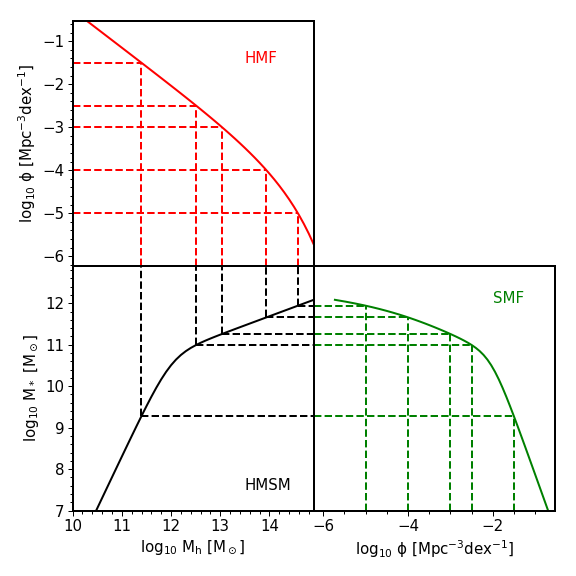
\includegraphics[width = \linewidth]{Figures/Chapter2/AbundaceMatching.png}
    \caption{A cartoon to show by matching the HMF (top left) and the SMF (bottom right) by abundance and the mapping between stellar and halo mass referred to as a SMHM relation (bottom left) is created.}
    \label{fig:Abn_Toon}
\end{figure}

The abundance matching used in \steel extracts central haloes from the halo mass function from \citet{Despali2016TheDefinitions} obtained using \textsc{colossus}\cite{Diemer2018COLOSSUS:Halos}, and a subhalo mass function subdivided by the redshift of infall generated from the statistical dark matter accretion history used by \textsc{steel}. Sub-haloes are assumed to follow the central SMHM relation at infall. We simplify our abundance matching by using a frozen model such that baryonic evolution after infall (stripping, star formation, etc.) is not included. The latter assumption provides a good approximation as after infall the dominant factor determining the abundances of satellite galaxies is the dynamical time and not evolutionary processes (Paper \RomanNumeralCaps{1}).

To fit stellar mass functions over multiple epochs we convolve our halo mass functions with a parametric SMHM relation similar to that proposed by \cite{Moster2010},
\begin{equation}
\label{eqn:MosAbn}
\begin{split}
M_*(M_h, z) &= 2M_hN(z)\Big[ \Big( \frac{M_h}{M_{n}(z)}\Big) ^{- \beta(z)} + \Big( \frac{M_h}{M_{n}(z)}\Big)^{\gamma(z)} \Big ]^{-1}\\
N(z) &= N_{0.1} +N_z\Big(\frac{z-0.1}{z+1}\Big)\\
M_{n}(z) &= M_{n,0.1} +M_{n,z}\Big(\frac{z-0.1}{z+1}\Big)\\
\beta(z) &= \beta_{0.1} +\beta_z\Big(\frac{z-0.1}{z+1}\Big)\\
\gamma(z) &= \gamma_{0.1} +\gamma_z\Big(\frac{z-0.1}{z+1}\Big).
\end{split}
\end{equation}

In what follows we create SMHM relations using both the cmodel and PyMorph SMF described in Section \ref{subsec:SMF} at redshift $z=0$ to constrain the parameters N, M, $\beta$, and $\gamma$ (normalization, knee, low mass slope, and high mass slope). We use only the central stellar mass function, using the \cite{Yang2012EvolutionHalos} central/satellite identification, and central halo mass function. The fit is performed using a Markov Chain Monte Carlo (MCMC)\footnote{In actuality the fit is first done by hand correcting parameters one at a time and visualised at each step. In doing so an appreciation of the connection between parameter value, SMHM shape, and SMF is built that promotes an in-depth understanding of the system and its caveats. Around the minimum value a brute force search is performed with various ranges and resolutions, this provides a test of the fit estimator that will be included in the MCMC. Once the limitations of the method are known building the MCMC is more robust as sensible checks and balances are included. The MCMC will often provide a solution close to the one found by the previous methods but find the robustness/errors associated with the result.}, implemented using the \textsc{python} package \textsc{emcee} \citep{Foreman-Mackey2013EmceeHammer}, over a large parameter space ($P_{M, N, \beta, \gamma}$) covering all four parameters. Given a point in parameter space $P_{M_i, N_i, \beta_i, \gamma_i}$, the stellar mass function is constructed using the halo mass function and the SMHM relation. Each bin of the central halo mass function is associated with a Gaussian distribution of stellar mass via the SMHM relation with scatter 0.15 dex. This distribution is multiplied by the halo mass number density to convert to galaxy number density which is added to the relevant stellar mass bins of the stellar mass function in construction. This operation is then repeated overall mass bins of the halo mass function to produce the complete central stellar mass function. For each point, $P_{M_i, N_i, \beta_i, \gamma_i}$ in the parameter space, the stellar mass function associated to that point is compared via a likelihood function to the observed stellar mass function to provide the MCMC with the probability that the given point is the `true' SMHM relationship. 

In Figure \ref{fig:Gauss_build} the above process is visualised, stripes in halo mass function are selected as shown in the left hand plot and then again in the middle as red bands. By propagating these bins of halo mass through the SMHM relation and associated scatter they each create a Gaussian of stellar mass as shown by overlapping green shading in the middle panel. Once weighted by the median halo number density they are added as green solid lines in the rightmost panel. Summing up each of the Gaussians created an estimation of the stellar mass is achieved. This figure is available animated at \url{https://twitter.com/RSEGrylls/status/1231279549704474624}. From this figure we see several features of the SMHM relation:
\begin{itemize}
    \item From the visualisation it can be seen that the scatter in the SMHM relation has two major effects: Firstly it can smooth out jaggedness introduced by the binning, one should therefore ensure that the scatter parameter is not influenced by the size of the binning to ensure results are physical and not numerical artefacts; Secondly the scatter dictates the size of the stellar mass gaussians it therefore dictates the range of stellar masses within a given halo mass bin. The width of the scatter has a second effect whereby lower mass halo bins can contribute to higher mass stellar mass bins this is known as 'upscatter', due to the greater number densities of lower mass haloes this can greatly impact the number densities of massive galaxies. This can be seen at high stellar masses where the peak of the stellar mass distribution sits below the previous distribution, this is the reason the scatter and the high mass slope are degenerate parameters when crating massive galaxies.
    \item It can be seen from the animated figure or by tracing haloes of mass $~10^{12}$ though the middle panel that the knee of the SMHM relation is closely related to the high mass cutoff in the SMF.
    \item Due to the fact that the high mass slope of the SMHM relation is much shallower than the low mass slope we see that the stellar mass distributions created are far more clustered and thus the high mass slope dictates a much smaller range of galaxies than the low mass slope.
\end{itemize}

\begin{figure}[h]
    \centering
    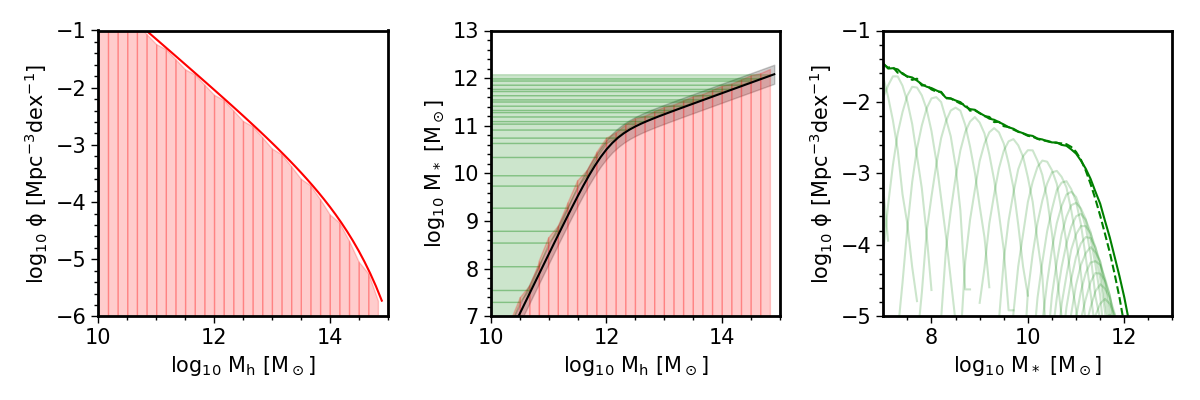
\includegraphics[width = \linewidth]{Figures/Chapter2/gaussian_buildup.png}
    \caption{A cartoon to show how the 'statistical' approach can be taken to transform a HMF to a SMF via number density propagation. From lest to right: Halo mass function with selected binning shown by shaded bands; The SMHM relation with the halo mass bins shown as red bands and the associated stellar mass distributions shown as green bands; The SMF with the Gaussian distributions from each halo mass bin shown as solid green curves that are then summed to create the total stellar mass function. An animated version of this plot made public by PJG can be found at \url{https://twitter.com/RSEGrylls/status/1231279549704474624}.}
    \label{fig:Gauss_build}
\end{figure}

We then fit to the \cite{Davidzon2017TheSnapshots} data both uncorrected and corrected for the cmodel and PyMorph fits respectively (see Section \ref{subsec:SMF} for details). At high redshift we use the central and subhalo mass functions initialising satellites at infall as described above\footnote{Ideally, as for low redshift, we would use the centrals only as we are primarily concerned with the central SMHM relation. However, lacking a well-defined central stellar mass function at high redshift, this method represents a reliable way to extend the model to higher redshifts.}. For central haloes the method is the same as detailed above, however, as we use the total stellar mass functions at high redshift we also include the total unevolved surviving subhalo mass function in the abundance matching. 
We assume that a halo before infall hosts a central galaxy; under this assumption we use the central SMHM relation to assign satellite galaxy stellar mass at the point of accretion. For the latter, we must have information about the redshift of infall for subhaloes. We obtain from \textsc{steel} the unevolved surviving subhalo mass function as contributed by each redshift of infall. Each contributing part is calculated using the SMHM relation at the redshift of infall and added to the central stellar mass function using the same method as with the centrals. The total stellar mass function is compared, at each redshift step available, to the data via the likely-hood function to give the probability that the given point is the `true' evolution parameters. The abundance matching best-fit parameters and associated errors for both the cmodel and PyMorph are given in Table \ref{tab:AbnResult}, and plots showing the cross-sections of the parameter space are shown in Appendix \ref{Appx:AbnMCMC}.

\begin{table}
\centering
\begin{tabular}{l||llll|llll}
        & $M_n$ & $N$     & $\beta$ & $\gamma$ & $M_{n,z}$ & N\_z   & $\beta_z$ & $\gamma_z$ \\ \hline
\\
cmodel  & $11.91_{-0.34}^{+0.40}$ & $0.029_{-0.013}^{+0.018}$ & $2.09_{-1.02}^{+1.21}$    & $0.64_{-0.10}^{+0.11}$     & $0.52_{-0.19}^{+0.24}$       & $-0.018_{-0.004}^{+0.005}$ & $-1.03_{-0.34}^{+0.049}$     & $0.084_{-0.14}^{+0.20}$      \\
\\
PyMorph & $11.92_{-0.36}^{+0.39}$ & $0.032_{-0.012}^{+0.016}$ & $1.64_{-0.73}^{+0.85}$     & $0.53_{-0.11}^{+0.11}$     & $0.58_{0.19}^{+0.15}$        & $-0.014_{-0.006}^{+0.007}$ & $-0.69_{-0.36}^{+0.29}$      & $0.03_{-0.147}^{+0.154}$      
\end{tabular}
\caption{The abundance matching results for the cmodel and PyMorph data. The errors are the 16th and 86th percentile from the MCMC fiting.}
\label{tab:AbnResult}
\end{table}

\begin{figure}[h]
    \centering
    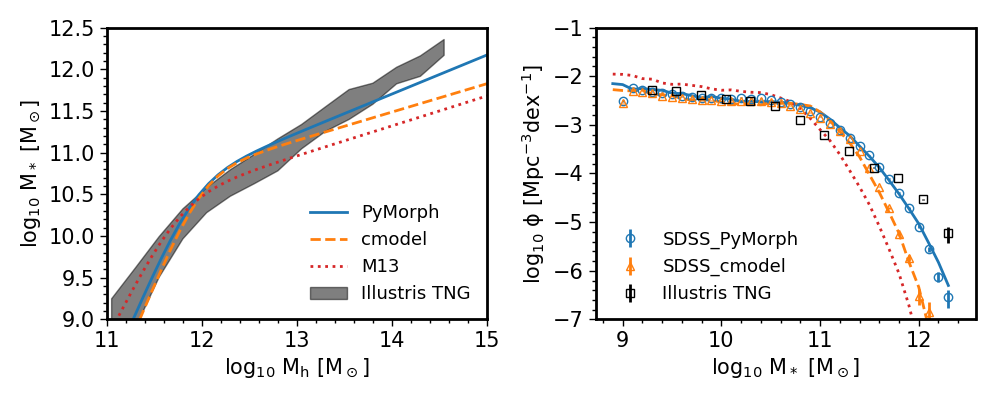
\includegraphics[width = \linewidth]{Figures/Chapter2/AbundaceMtch_Data.png}
    \caption{Left: The SMHM relation at redshift $z=0.1$. The PyMorph (blue solid line) and cmodel (orange dashed line) fits from this work are both for central haloes/galaxies, the fit from \citet{Moster2013} (M13, red dotted line) is for all haloes/galaxies. The grey band is the relation from Illustris TNG100. Right: Stellar mass functions created using the central halo mass function and the three SMHM relations compared to PyMorph (blue circles) and cmodel (orange triangles) central stellar mass functions. The black squares are the stellar mass function from Illustris TNG100.}
    \label{fig:Abn_Data}
\end{figure}

In Figure \ref{fig:Abn_Data} we show the results of our abundance matching to the PyMorph and cmodel central stellar mass functions. The PyMorph fit is steeper above the knee compared to either the cmodel or the \citet{Moster2013} model fits, as expected given the larger number density of massive galaxies found applying the S\'ersic-Exponential model \citep[eg.,][]{Shankar2014, Kravtsov2018StellarHalos}. The low mass slope for both PyMorph and cmodel are almost identical as the galaxies in this range are not affected by the photometric choice. Differences between the fits from this work and \citet{Moster2013} are due to our selection of using only central haloes/galaxies as opposed to the total population, and the stellar mass functions shown in the right-hand panel are lower than even cmodel are therefore missing massive galaxies.


\subsection{Continuity star formation rate}

A substantial modelling problem arises from the continuity between the evolution of the SMF and the observed SFR. The observed UV star formation rates applied to high redshift stellar mass functions when evolving populations conserving number density between epochs yield stellar mass functions higher than those observed. This deviation led to models which can not simultaneously reproduce the observed SFR and SMF, without invoking harsh feedback routines.

\begin{figure}[h]
    \centering
    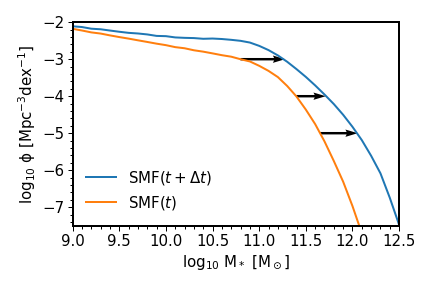
\includegraphics[width = \linewidth]{Figures/Chapter2/ContinuityEqn.png}
    \caption{The continuity approach connects at constant number density galaxy populations across cosmic time. Between two epochs `$t$' and `$t + \Delta t$' the SMF grows differently at different number density. The mass difference, $\Delta M$, indicated at three number densities by black arrows is the expected mass growth for each population.}
    \label{fig:Cont_Eqn}
\end{figure}

The continuity star formation rate is a theoretical quantity calculated such that the observed growth of the stellar mass function is conserved. As illustrated in Figure \ref{fig:Cont_Eqn} by connecting two SMF at consistent number density at times `$t$' and `$t + \Delta t$' the growth in mass $\Delta M$ at each number density over the time $\Delta t$ is obtained. In the simplest approximation, the SFR is equal to $\Delta M / \Delta t$. However, the observed star formation rate is higher than the this value. As new stars are created a proportion of the mass is recycled through supernova `quickly' in terms of cosmological time. This mass recycling given in \citet{Moster2018Emerge10} is used to amend the star formation rate, to account for the mass loss based on the entire star formation history of the galaxy. The fraction of mass lost by a population of stars over time $\tau_{ml}$ is given by,

%Mass recycling
\begin{equation}
\label{eqn:f_ml}
f(\tau_{ml}) = 0.05 \ln \Big(\frac{\tau_{ml}}{1.4 Myr}+1\Big),
\end{equation}

summing the difference in fraction lost in a time step $\delta t$ for every star formation epoch in the galaxies history (SFH) gives the mass loss rate (MLR), 

\begin{equation}
\label{eqn:MLR}
MLR(t) = \frac{ \sum_{t' = t_{inf}}^{t} SFH(t')(f[t' - (t-\delta t)]-f[t' - t]) }{\delta t}.
\end{equation}

The continuity SFR is therefore calculated to be $\Delta M / \Delta t$ + MLR. The final correction made to this star-formation rate is that galaxies also accrete mass via mergers this accrete mass term ($M_{acc}$) is prominent for massive galaxies $M_* > 10^{11} M_{\odot}$. The continuity SFR at time t' is then finally,

\begin{equation}
    SFR_{continuity}(t') = \frac{\Delta M(t')}{\Delta t} + MLR(t') - M_{acc}(t').
\end{equation}

\subsection{Empirical central galaxy growth}

Using the stellar-mass-halo-mass (SMHM) relation and halo mass growth histories (HMGH) we make an empirical prediction of the average central galaxy growth. In Figure \ref{fig:Cent_Mass_PP} we show in the top left the HMGH for two haloes $M_{z=0} = 10^{14}, 10^{12.5} M_{\odot}$, the middle panel shows the SMHM where the shading shows the extent of the evolution of the median of the relation over the redshift range, finally the bottom left shows the stellar mass growth history (SMGH) predicted by the latter two inputs.

%include a plot of using AM to convert HMGH to SMGH?
\begin{figure}[h]
    \centering
    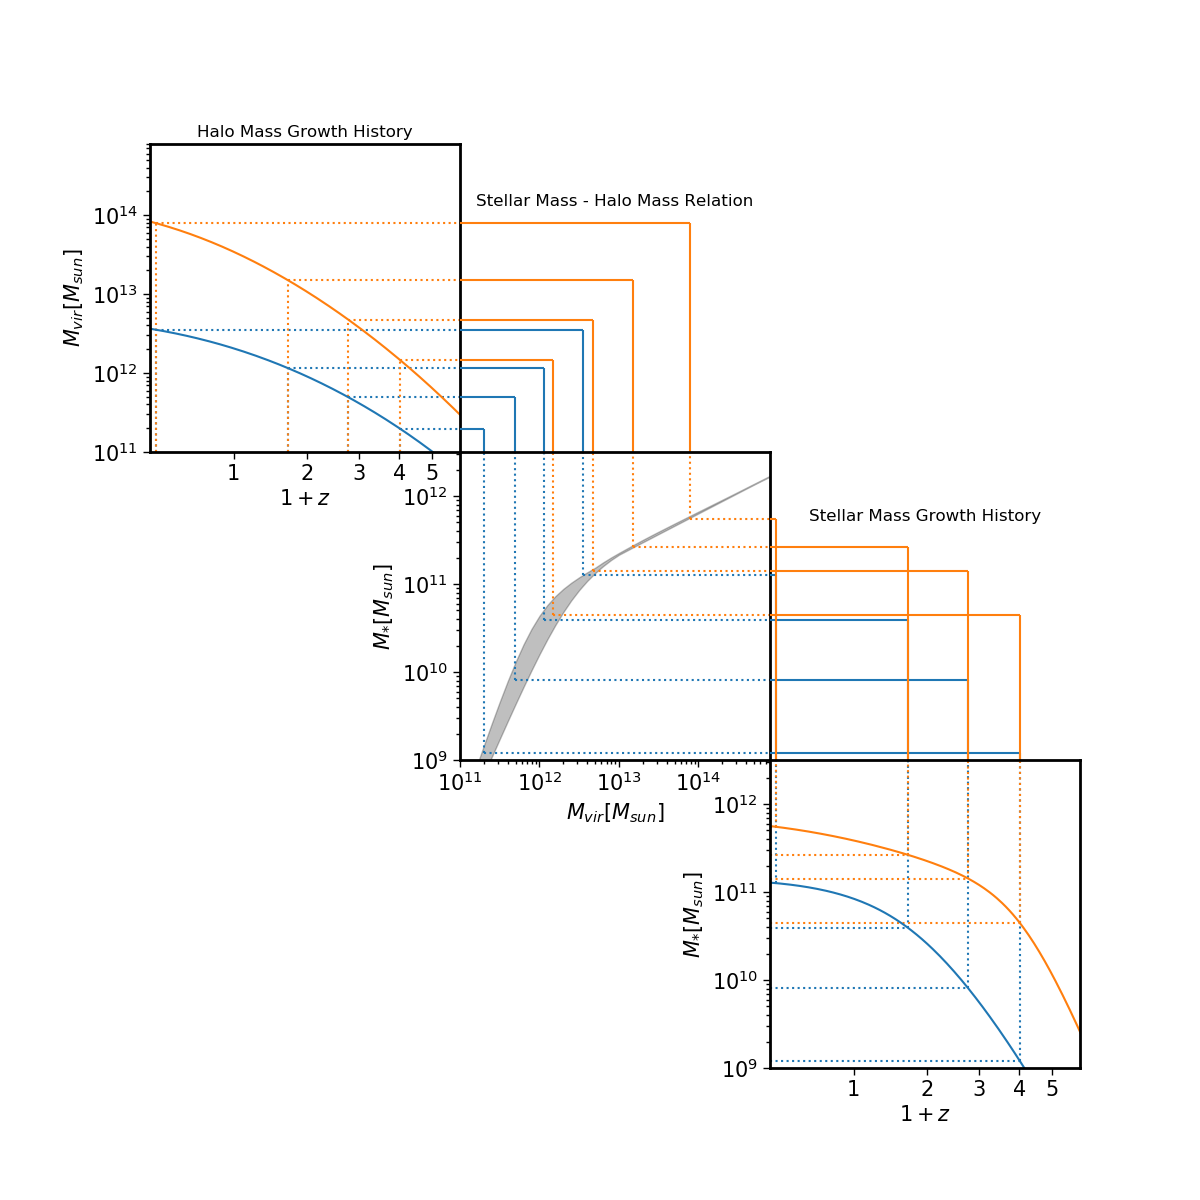
\includegraphics[width = \linewidth]{Figures/Chapter2/HMGH_to_SMGH.png}
    \caption{The Halo Mass Growth Histories (HMGH, top-left) are propagated through the redshift dependent stellar-mass-halo-mass relation (SMHM, middle) to produce corresponding Stellar Mass Growth Histories (SMGH, bottom-right). The lines illustrate matching points in redshift and the intersection with the SMHM relationship. The width of the SMHM relationship shows the extent of evolution with time, not as is common the scatter.}
    \label{fig:Cent_Mass_PP}
\end{figure}

At several redshift epochs, the HMGH to the SMGH are connected following the colour-coded lines, it is found the shape of the SMHM relationship is the primary factor that dictates the shape of the SMGH. Identifying for each growth history the step before the central galaxy growth rapidly slows $z = 3$ for orange and $z = 1$ for blue each of these lines intersect the HMGH when it is still growing, whereas they intersect the SMHM relationship just before the `knee'. This change in the growth behaviour is thought to be an effect of active galactic nuclei suppressing the formation of stars in a galaxy. However, as the knee is a function of halo mass once could also attribute this to the halo mass at which infalling gas is shock heated and can no longer efficiently accrete to the central galaxy.

\section{Discussion}

This chapter has outlined the core methodologies of \steel as they stood at the time of writing. For exact details of the development of the methods we refer the reader to the full papers in Appendix \ref{Appx:Papers}. For example, the continuity star formation rate in \Paper{1} was derived by generating SMF at subsequent time-steps and then following populations at consistent number density; In \Paper{2} the method was updated to instead follow the central dark matter growth histories. 

At it's inception \steel was a short test script we were using to try to test what the maximum number of satellites in a halo given a SMHM relation. The 75 line code in Section \ref{sec:Proof} is a recreation of the original script with additional formatting and commenting\footnote{Note this script will not run as the SMHM relation called from SEM is not present neither are the parameters to be sent to that script. The naming conventions are as originally used being a patchwork of other scripts. trapz is a simple trapezium integrator that would also need to be replaced. This script is unlicensed and only intended as a guide to the original thoughts that went into building the foundation of \steel}.

\section{Future}

As will be seen in the following Science Chapters (3, 4, \& 5) the novelty of \steel provides a view on galaxy formation physics that can refresh and re-frame some ideas in the field. However, as \steel grew naturally from the proof of concept, it has now reached a stage common to many software programs where it requires a critical tear down and refactor. Developing \steel is possible only for PG and those trained by PG without a significant time investment, therefore a refactor will provide the following usability and science benefits. 
\begin{itemize}
    \item Development ease: A redesign of the software architecture will make the addition of new modules easier important for retaining flexibility.
    \item Method: Many of the routines in steel involve weighted statistical distributions (mostly small gaussian scattering) it would therefore be in the interests of the model to redesign the methodology around an object orientated approach that handles many probability distribution convolutions by design.
    \item Speed: \steel is much faster than most models as is the design spec, however, the choice of \textsc{python} as the language has had certain drawbacks.  Iterative process are slow, for this reason the entire starformation module was written in \textsc{cython} a type defined version of python that is pre-compiled into \textsc{c}, this process is both slow and difficult. With a full refactor the choice of language and acceleration tools could be more carefully considered with the end product known.
    \item Science: Many requests have been made of \steel by others recognising it as a potentially revolutionary tool, some are possible but hard, for example adding gas fractions requires a 4th dimension to be added to the running/output data. Others are (near)impossible under the current logic of the code such as creating partitions in the central population and treating each population differently. These again could be designed into a full refactor.
    \item Output: The data output from \steel and the 'post-processing' modules are messy. The simple initial models could save files by name with only 9(/18) parameter combinations that were of interest. This has not scaled well and a full rethink of the data handling, model launching, and output plotting is sorely required.
    \item Integration: Relying on all the above \steel has been proposed by PJG as a necessary analysis tool for ensuring the self consistency of future extra-galactic surveys. Further details will be given in Chapter \ref{Chapter:Conclusion} and a technical outline can be found in Appendix \ref{Appx:HF} where a 4 year fellowship outline of work can be found.
\end{itemize}

\pagebreak
\section{Proof of concept}
\label{sec:Proof}
\inputminted{python}{Codes/Proof.py}
